\section{Vorbereitung}
 {Die Versuchsvorbereitung ist Bestandteil des Versuchs. Sie erhalten dafür ein gesondertes Testat.
  Ohne testierte Vorbereitung können Sie den Versuch nicht durchführen.}
\subsection{Ersatzschaltbild Transformator}
\begin{enumerate}[label=\alph*)]
	\item Zeichnen Sie das vollständige einphasige Ersatzschaltbild (Sternschaltung) des
	      Transformators und geben Sie an, wie die einzelnen Werte und das
	      Übersetzungsverhältnis ü aus dem Leerlauf- und dem Kurzschlussversuch berechnet
	      werden können.
	      \begin{figure}[h!]
		      \begin{center}
			      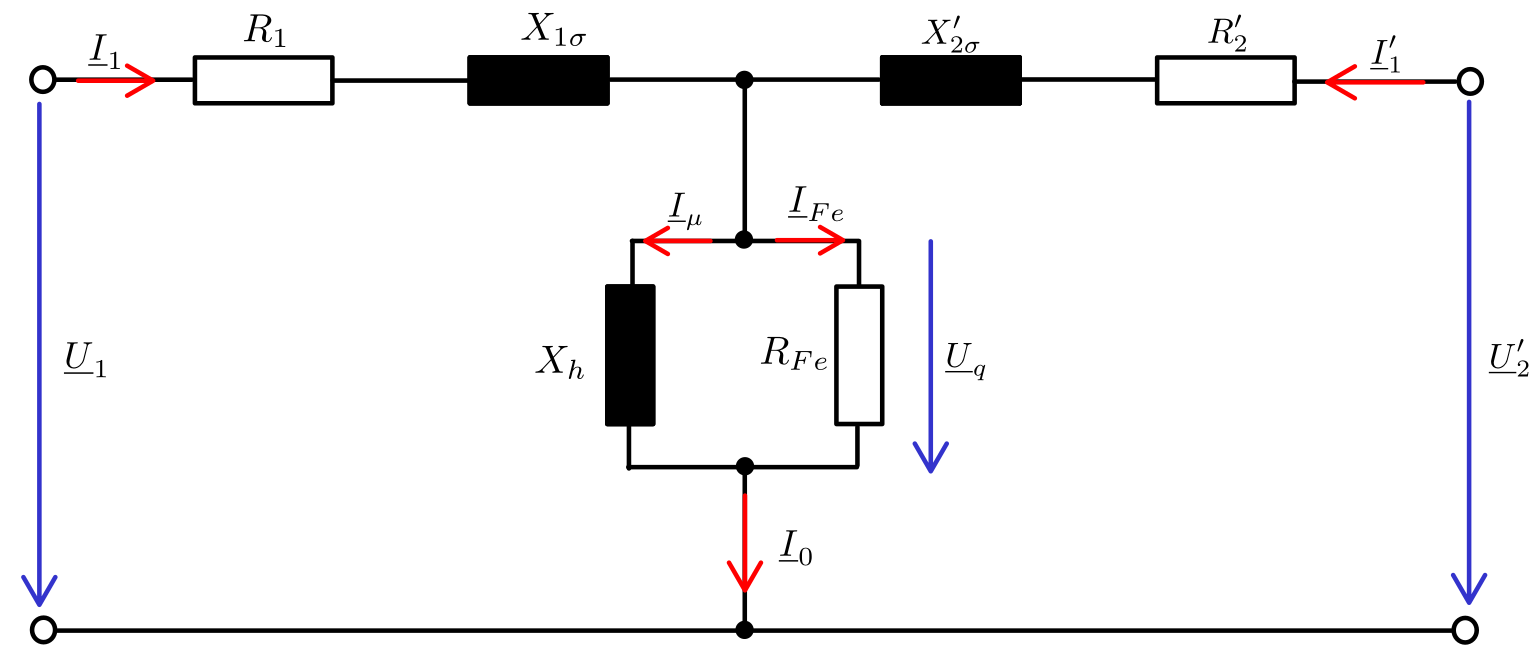
\includegraphics[width=0.95\textwidth]{img/2.1.1.1}
		      \end{center}
		      \caption{Vollständige einphasige Ersatzschaltbild des Transformators}\label{img:2.1.1.1}
	      \end{figure}
	      $$ü=\frac{U_1}{U_2}=\frac{w_1}{w_2}=\frac{I_2}{I_1}$$
	      \begin{minipage}{0.5\textwidth}
		      Leerlauf:
		      \begin{align*}
			      R'_2         & =R_2\cdot ü^2           \\
			      U'_2         & =U_2\cdot ü             \\
			      I'_2         & = \frac{I_2}{ü}         \\
			      X'_{2\sigma} & = X_{2\sigma} \cdot ü^2 \\
			      P'_2         & = P_2
		      \end{align*}
	      \end{minipage}\hfill
	      \begin{minipage}{0.5\textwidth}
		      Kurzschluss:
		      \begin{align*}
			      R_K     & = R_1 + R'_2                 \\
			      X_K     & = X_{1\sigma} + X'_{2\sigma} \\
			      Z_K     & = \sqrt{R_K^2 + X_K^2}       \\
			      U_{R_K} & = R_K \cdot I_1              \\
			      U_{X_K} & = X_K \cdot I_1
		      \end{align*}
	      \end{minipage}

	      \pagebreak
	\item Machen Sie sich die Bedeutung der einzelnen Bauelemente des vollständigen
	      Ersatzschaltbildes klar (wird abgefragt). Welche Bedeutung haben die
	      „gestrichenen“ Größen?
	      \begin{figure}[h!]
		      \begin{center}
			      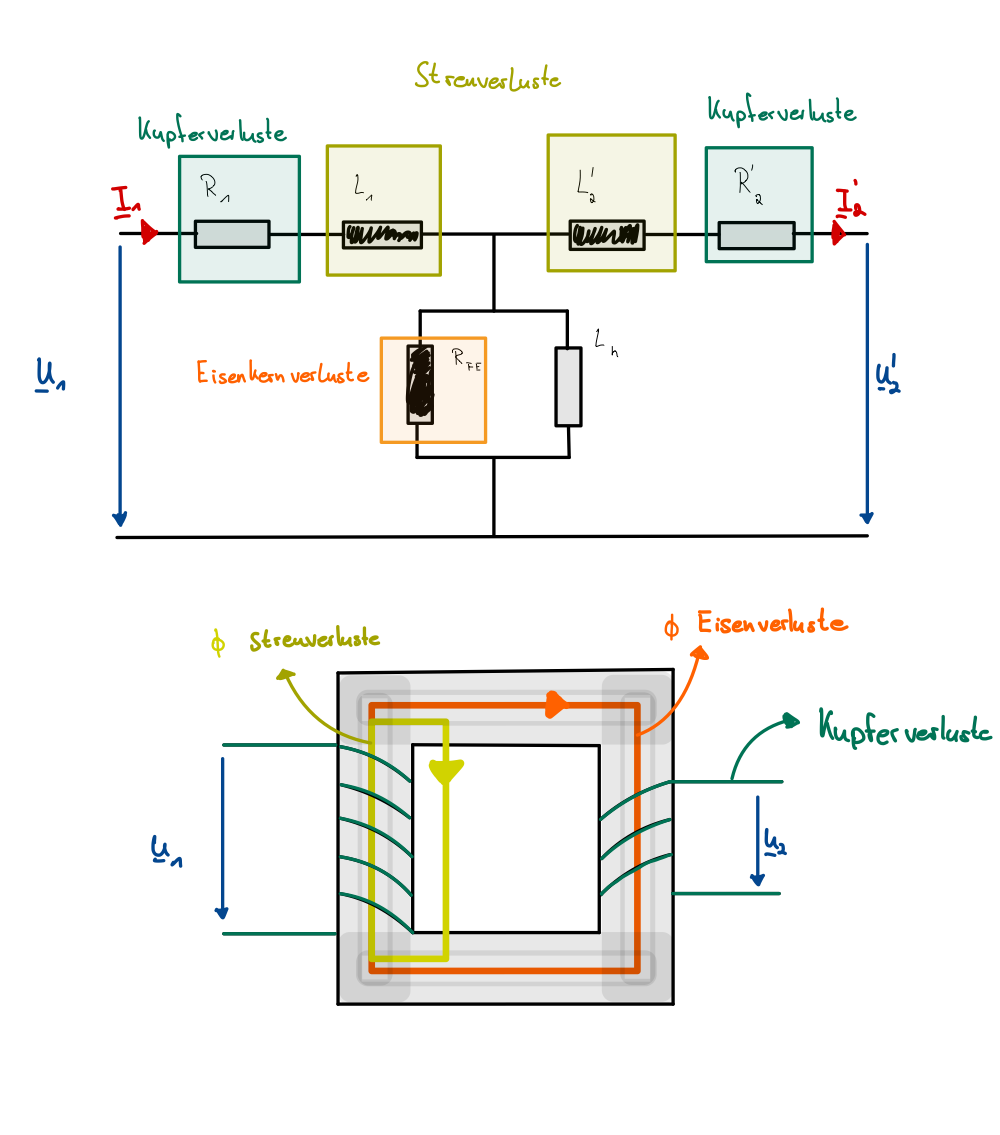
\includegraphics[width=0.8\textwidth]{img/2.1.2.4.png}
		      \end{center}
		      \caption{Zeichnung der eines Realentransformators mit Schaltpan }\label{img/2.1.2.4}
	      \end{figure}
	      \\
	      Das Ersatzschaltbild besteht aus verschiedenen Verlustkomponenten. Der Eisenkern bewirkt
	      Energieverluste aufgrund von Hysterese und Wirbelströmen, die im Kern erzeugt werden. Sowohl
	      an den Primär- als auch an den Sekundäranschlüssen befinden sich Kupferwicklungen, die aufgrund
	      ihrer Länge ohmsche Verluste erzeugen, insbesondere unter Wechselstrombedingungen, wo Stromverdrängungseffekte
	      auftreten. Der magnetische Fluss erstreckt sich nicht nur durch den Eisenkern, sondern breitet sich auch durch
	      die Umgebungsluft aus, was zu einem Streufluss führt. Dieser Streufluss trägt nicht zur Energieübertragung bei.\\ \ \\

	      Die Striche an den Bauteilen signalisieren, dass diese bereits transformiert
	      sind. Um die Spannung und den Strom umzuwandeln, muss das Ersatzschaltbild um
	      einen idealen Transformator auf der Sekundärseite erweitert werden, da allein
	      passive Bauelemente keine Transformationsfunktion erfüllen können.\\

	\item Wie groß darf der Strom im Kurzschlussversuch maximal werden? Begründen Sie
	      Ihre Aussage.\\ \ \\

	      Im Kurzschlussversuch bei einem Transformator wird die Eingangsspannung
	      schrittweise erhöht, bis der Strom auf der Primärseite den Nennstrom $(I_{1N})$
	      erreicht. Dabei muss beachtet werden, dass der Kurzschlussversuch eine Art von
	      Überlasttest ist, und es ist wichtig, die zulässigen Grenzen einzuhalten, um
	      Schäden am Transformator zu vermeiden.
	      \[ I_K = I_{1N} \]
	      Die maximale Strombelastung im Kurzschlussversuch wird durch die thermische
	      Belastung des Transformators begrenzt. Wenn der Strom zu hoch wird, kann dies
	      zu übermäßiger Erwärmung führen, was zu Isolationsversagen oder anderen Schäden
	      führen kann. Daher sollte der Kurzschlusstest so durchgeführt werden, dass der
	      Transformator nicht beschädigt wird.

	      Der Strom im Kurzschlussversuch sollte normalerweise auf einen Wert begrenzt
	      werden, der sicher unterhalb des Kurzschlussspitzenstroms $(I_{k})$ liegt. Der
	      Kurzschlussspitzenstrom tritt aufgrund von Transienten auf, wenn der
	      Transformator plötzlich kurzgeschlossen wird. Er kann ein Vielfaches des
	      Nennstroms betragen und ist kurzzeitig.

	      Die genaue maximale zulässige Strombelastung im Kurzschlussversuch hängt von
	      den spezifischen Eigenschaften des Transformators ab, einschließlich seiner
	      Größe, Bauart und Kühlung. Herstellerangaben und Normen sollten für eine genaue
	      Bestimmung konsultiert werden. Es ist wichtig, den Kurzschlussversuch
	      sorgfältig zu planen und sicherzustellen, dass er den Spezifikationen des
	      Transformators entspricht, um Schäden zu vermeiden und die Sicherheit zu
	      gewährleisten.

	\item Leiten Sie her, wie die Verlustleistung des Transformators in einem beliebigen
	      Betriebspunkt (vorgegeben durch den Strom $I_1$) aus den Verlusten der
	      Leerlauf- und Kurzschlussmessung ermittelt werden kann.

	      \begin{align*}
		      P_{Cu}               & = P_K\cdot \frac{I^2}{I^2_N}\mspace{100mu} |P_K\ =\ 3\cdot R_K\cdot I^2_N \\
		      P_{Cu}               & = 3\cdot R_K\cdot I^2_N\cdot \frac{I^2}{I^2_N}                            \\
		      P_{Cu}               & = 3\cdot R_K\cdot I^2                                                     \\
		      \\
		      P_{Fe}               & = P_0\cdot \frac{U^2}{U^2_N}\mspace{100mu} |P_0\ =\ \frac{U^2_N}{R_{Fe}}  \\
		      P_{Fe}               & = \frac{U^2_N}{R_{Fe}}\cdot \frac{U^2}{U^2_N}                             \\
		      P_{Fe}               & = \frac{U^2}{R_{Fe}}                                                      \\
		      \\
		      \Longrightarrow\ P_V & = 3\cdot R_K\cdot I^2\ +\ \frac{U^2}{R_{Fe}}
	      \end{align*}

	\item Leiten Sie anhand des Zeigerdiagramms (Bild 6) die Formeln für den Längs- und
	      Querspannungsabfall her.
	      \begin{align*}
		      \underline{\Delta U} & = \underline Z\cdot \underline I_1                                                                                                        \\
		      \underline{\Delta U} & = (R_k+ jX_k)\cdot (I_1\cdot e^{-j\varphi_2})                                                                                             \\
		      \underline{\Delta U} & = (R_k+ jX_k)\cdot \left(I_1\cdot\cos(-\varphi_2)+j\cdot I_1\cdot \sin(-\varphi_2)\right)                                                 \\
		      \underline{\Delta U} & = (R_k+ jX_k)\cdot \left(I_1\cdot\cos\varphi_2-j\cdot I_1\cdot \sin\varphi_2\right)                                                       \\
		      \underline{\Delta U} & = R_K\cdot I_1\cdot \cos\varphi_2 + X_K\cdot I_1 \cdot \sin\varphi_2+J(-R_K\cdot I_1 \cdot \sin\varphi_2+X_K\cdot I_1\cdot \cos\varphi_2) \\
		      \underline{\Delta U} & = U_\ell +jU_q                                                                                                                            \\
		      \Rightarrow U_\ell   & =Re{\underline{\Delta U}}=R_K\cdot I_1 \cdot\cos \varphi_2 + X_K \cdot I_1\cdot \sin \varphi_2                                            \\
		      \Rightarrow U_q      & =Im{\underline{\Delta U}}= -R_K\cdot I_1 \cdot\sin \varphi_2 + X_K \cdot I_1\cdot \cos \varphi_2                                          \\
	      \end{align*}
	\item Leiten Sie anhand des Zeigerdiagramms (Bild 6) und den Formeln für den Längs-
	      und Querspannungsabfall die Formel (12) für den relativen Spannungsfall auf der
	      Sekundärseite her.
	      \begin{align*}
		      \Delta U'_2                            & = \frac{U_1 - U'_2}{U_1}                                                                                                \\
		      \Delta U'_2                            & = 1-\frac{U'_2}{U_1}                                                                                                    \\
		      \underline U'_2+\underline U_\ell      & = \sqrt{\underline U_1^2-\underline U_q^2}                                                                              \\
		      \underline U'_2                        & = \sqrt{\underline U_1^2-\underline U_q^2}-\underline U_\ell                                                            \\
		      \frac{\underline U'_2}{\underline U_1} & = \frac{\sqrt{\underline U_1^2-\underline U_q^2}}{\underline U_1}-\displaystyle\frac{\underline U_\ell}{\underline U_1} \\
		      \frac{\underline U'_2}{\underline U_1} & = {\sqrt{\frac{\underline U_1^2-\underline U_q^2}{\underline U_1^2}}}
		      -\displaystyle\frac{\underline U_\ell}{\underline U_1}                                                                                                           \\
		      \frac{\underline U'_2}{\underline U_1} & = {\sqrt{1-\left(\frac{\underline U_q}{\underline U_1}\right)^2}}
		      -\displaystyle\frac{\underline U_\ell}{\underline U_1}                                                                                                           \\
		      \Delta U'_2                            & = 1-\frac{U'_2}{U_1}                                                                                                    \\
		      \Delta U'_2                            & = 1 + \frac{U_\ell}{U_1}- \sqrt{1-\left(\frac{U_q}{U_1}\right)^2}
	      \end{align*}
	\item Welche Aussagekraft hat die relative Kurzschlussspannung für den Betrieb des
	      Transformators?

	      Die relative Kurzschlussspannung eines Transformators ist ein entscheidender
	      Parameter, der seine Verhaltensweise unter Belastung widerspiegelt. Dieser Wert
	      ist von großer Bedeutung bei der Auslegung von Niederspannungsverteilungen
	      sowie bei der Dimensionierung von Komponenten wie Sicherungsleisten und
	      Leistungsschaltern.

	      Die relative Kurzschlussspannung gibt an, wie stark die Spannung ansteigt, wenn
	      die Sekundärseite des Transformators kurzgeschlossen wird und der Nennstrom auf
	      der Sekundärseite fließt. Dies ist von Bedeutung, da im Falle eines
	      Kurzschlusses in der Verteilung die Sekundärseite des Transformators weiterhin
	      am Netz angeschlossen ist, bis der vorgeschaltete Schutzmechanismus auslöst.

	      Die Kenntnis der relativen Kurzschlussspannung ermöglicht die Berechnung des
	      maximalen Kurzschlussstroms, der in diesem Szenario auftreten kann. Ein
	      einfacher Dreisatz kann verwendet werden, um dies zu ermitteln. Als Beispiel
	      kann ein Drehstromtransformator mit den Spezifikationen $6\ KV / 400\ V$ und
	      einer relativen Kurzschlussspannung von $6\ \%$ dienen. Der sekundäre Nennstrom
	      beträgt $145\ A$.

	      Die Berechnung des maximalen Kurzschlussstroms erfolgt durch die Division des
	      Nennstroms durch die relative Kurzschlussspannung in Prozent. In diesem Fall
	      ergibt sich ein Wert von $24\ A$. Dieser Strom, hier $2400\ A$, kann kurzzeitig
	      durch die nach dem Transformator geschalteten Schutzschalter fließen. Es ist
	      jedoch zu beachten, dass die dynamischen Kräfte, die bei einem Kurzschluss
	      auftreten, die Schaltelemente mechanisch belasten und sie gegebenenfalls
	      beschädigen können.

	      Es ist daher entscheidend, die Kurzschlussfestigkeit der verwendeten
	      Komponenten zu überprüfen und gegebenenfalls hochwertigere Komponenten
	      auszuwählen. In vielen Fällen sind gängige Niederspannungsschaltgeräte jedoch
	      für Kurzschlussströme von $6\ kA$ ausgelegt und erfüllen die Anforderungen.
\end{enumerate}

\subsection{Aronschaltung zur Leistungsmessung }
\begin{enumerate}[label=\alph*)]
	\item Leiten Sie her, warum Sie mit der Aronschaltung (Bild 8) die gesamte
	      Scheinleistung im Dreiphasensystem messen können, sofern der Summenstrom im
	      Knoten K zu Null angenommen werden kann.

	      \begin{figure}[h!]
		      \begin{center}
			      \begin{minipage}[ct]{0.4\linewidth}
				      \begin{center}
					      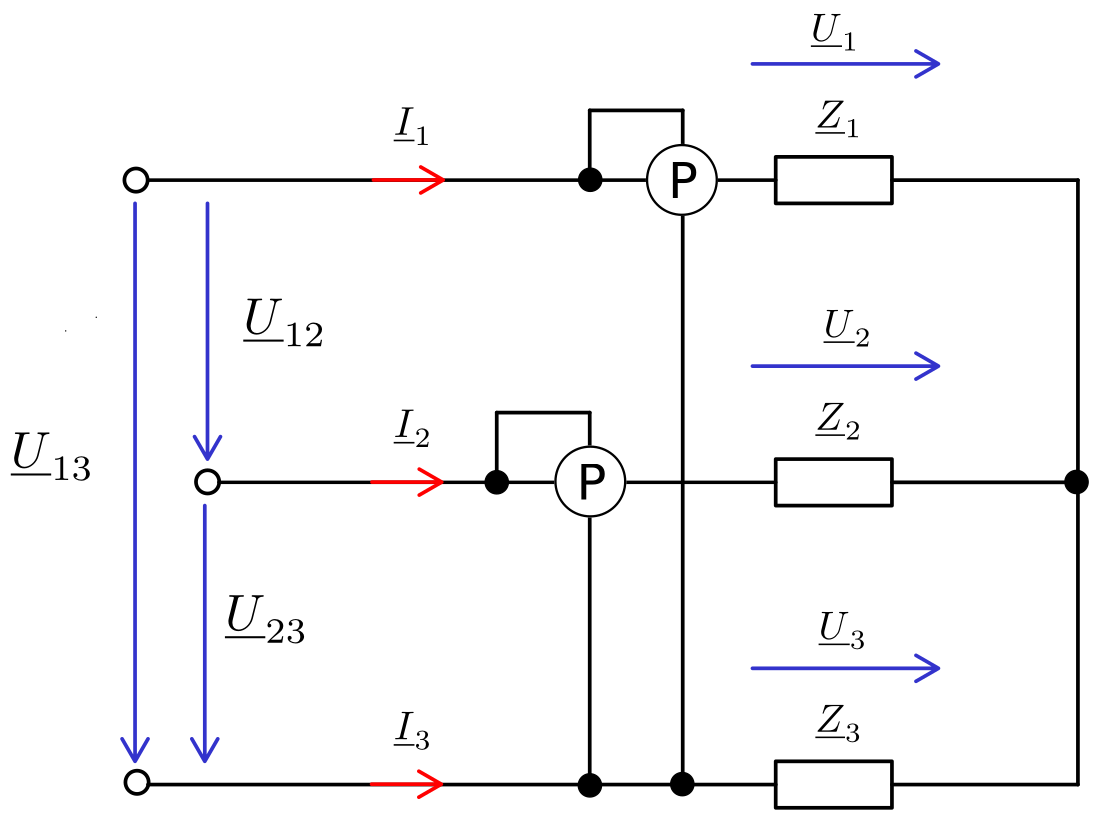
\includegraphics[width=\linewidth]{img/2.2.1.1.png}
				      \end{center}
				      \caption{Schaltplan von einem realen Transformator mit einem Lastwiderstand}\label{img/2.2.1.1}
			      \end{minipage}
			      \hspace{.1\linewidth}
			      \begin{minipage}[ct]{0.4\linewidth}
				      \begin{center}
					      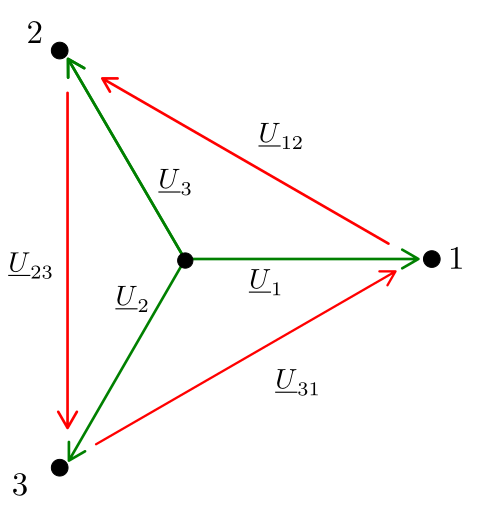
\includegraphics[width=\linewidth]{img/2.2.1.2.png}
				      \end{center}
				      \caption{Zeigerdiagram einer Sternschaltung}\label{img/2.2.1.2}
			      \end{minipage}
		      \end{center}
	      \end{figure}



	      \begin{align*}
		      \text{Kontenregel gilt: ges.:}\  \underline{i}_3                                                                                                                 \\
		      0               & =\ \underline{i}_1 + \underline{i}_2 + \underline{i}_3                                                                                         \\
		      \underline{i}_3 & = - \underline{i}_1 - \underline{i}_2                                                                                                          \\
		      \text{Leistungsgleichung:}                                                                                                                                       \\
		      \underline{S}   & =\ \underline{U} \cdot\ \underline{I}\ =\ \underline{u} \cdot \underline{i}                                                                    \\
		      \underline{S}   & =\ \underline{u}_1 \cdot \underline{i}_1 + \underline{u}_2 \cdot \underline{i}_2 + \underline{u}_3 \cdot \underline{i}_3                       \\
		      \underline{S}   & =\ \underline{u}_1 \cdot \underline{i}_1 + \underline{u}_2 \cdot \underline{i}_2 + \underline{u}_3 \cdot (- \underline{i}_1 - \underline{i}_2) \\
		      %S &= \ \underline{u}_1 \cdot \underline{i}_1 + \underline{u}_2 \cdot \underline{i}_2 - \underline{u}_3 \cdot \underline{i}_1 - \underline{u}_3 \cdot \underline{i}_2)\\
		      \underline{S}   & = \underline{i}_1(\underline{u}_1 - \underline{u}_3) + \underline{i}_2(\underline{u}_2 - \underline{u}_3)                                      \\
		      \underline{S}   & = \underline{i}_1\cdot\underline{u}_{13} + \underline{i}_2\cdot\underline{u}_{23}
	      \end{align*}
	      \begin{align*}
		      \text{Phasenverschiebungswinkel:}                                          \\
		      L_{M}\ =\ \text{Leistungsmessgerät}                                        \\ \ \\
		      +\ L_{M1}   & =\ +\ L_{M2}\ \ \ \ \{ \varphi =\ 0^\circ                    \\
		      +\ L_{M1}   & =\ -\ L_{M2}\ \ \ \ \{ \varphi =\ \pm90^\circ                \\
		      \ L_{M1}    & \neq\ \ L_{M2}\ \ \ \ \{ 0^\circ< \varphi < 60^\circ         \\
		      -\ L_{M1}\  & \text{oder}\ -\ L_{M2}\ \ \ \ \{ 60^\circ< \varphi < 0^\circ \\
	      \end{align*}
	\item Skizzieren Sie das Ersatzschaltbild für den Transformator im Leerlauffall.
	      Zeichnen Sie das zugehörige qualitative Zeigerdiagramm für den Leerlauffall.
	      \begin{figure}[h!]
		      \begin{center}
			      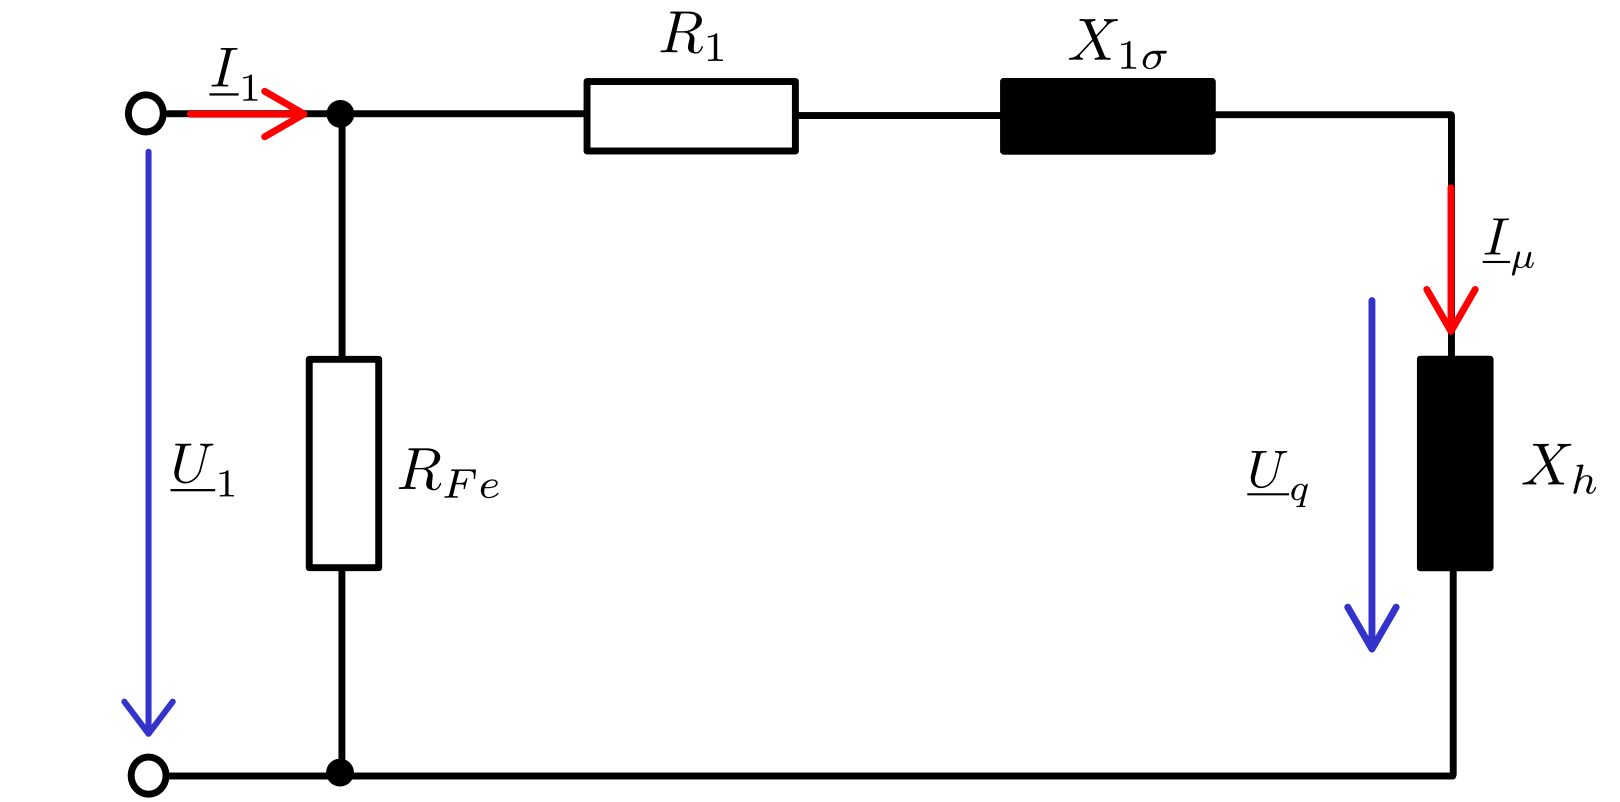
\includegraphics[width=0.95\textwidth]{img/2.2.2.1}
		      \end{center}
		      \caption{ESP für den Transformator im Leerlauffall}\label{img:2.2.2.1}
	      \end{figure}

	\item Zeigen Sie anhand dieses Zeigerdiagramms, warum Sie im Leerlaufversuch (Bild 9)
	      mit der Aronschaltung eine negative Wirkleistung P1 messen.
\end{enumerate}

\subsection{Symmetrische Drehstromlast }
\begin{enumerate}[label=\alph*)]
	\item Geben Sie an, wie Sie aus den Messwerten nach 3.2 (a) und (b) die gemittelten
	      Größen $U_m,\ I_m$ (siehe Versuch E2-4), den Leistungsfaktor
	      $\lambda=\cos(\varphi)$, die Leistungen $S,\ P\ und\ Q$ jeweils für die Primär-
	      und die Sekundärseite berechnen können.\\ \ \\ Leistungsfaktor $\lambda(\cos
			      (\varphi))$:
	      \[ \lambda = \frac{|P|}{S}=\frac{S\cdot |\cos \varphi|}{S} = |\cos \varphi| \]
	      Der Leistungsfaktor kann zwischen $0$ und $1$ liegen: $0 \leq \lambda \leq 1
	      $\\ Leistungen $S$, $P$ und $Q$:\\
	      \begin{align*}
		      P & = U_M\cdot I_M\cdot \lambda \\
		      S & = U_M\cdot I_M              \\
		      Q & = \sqrt{S^2-P^2}
	      \end{align*}

	\item Mit welcher Leistung können Sie den Transformator ($Yy0$) maximal belasten?
	      \begin{align*}
		      S_{max} & = \sqrt 3 \cdot U_{max}\cdot I_{max} \\
		      S_{max} & = \sqrt 3 \cdot 380\ \cdot 7,6\ A\\
          S_{max} & = 5\ \text{kVA}
	      \end{align*}
\end{enumerate}
